\section{Desarrollo del Sistema}
	
	Para el desarrollo del sistema se utilizó el siguiente stack de tecnologías
	(frontend y backend):
	
	\begin{itemize}
	  \item HTML y CSS (Bootstrap)
	  \item Javascript (AngularJS)
	  \item NodeJS (ExpressJS)
	  \item Java (Spring y Spring Boot)
	\end{itemize}
	
	\subsection{Arquitectura de Aplicaciones Web Modernas}
		A principios de la web, las ``aplicaciones web'' no existían. La web
  		consistía de contenido estático e imágenes.\\\
  
  		Ventajas:
  
  		\begin{itemize}
			\item Bajo consumo computacional en el servidor
			\item El contenido era facilmente Aumentar!!!!!  
		\end{itemize}
		
		Desventajas:
		
		\begin{itemize}
			\item Actualización de contenido engorroso
			\item Personalización inexistente, todas las personas que visitan la web, ven
			el mismo contenido
			
			\item Interfaz de usuario muy básica, comparado con las aplicaciones de hoy
		\end{itemize}
		
		Las aplicaciones web modernas estan compuestas de clientes frontend y una
		infraestructura backend distribuida (para servir contenido) a través del
		uso de APIs RESTful (figura \ref{figure:webapp-arq}).
		
		\begin{figure}[H]
		    \centering
			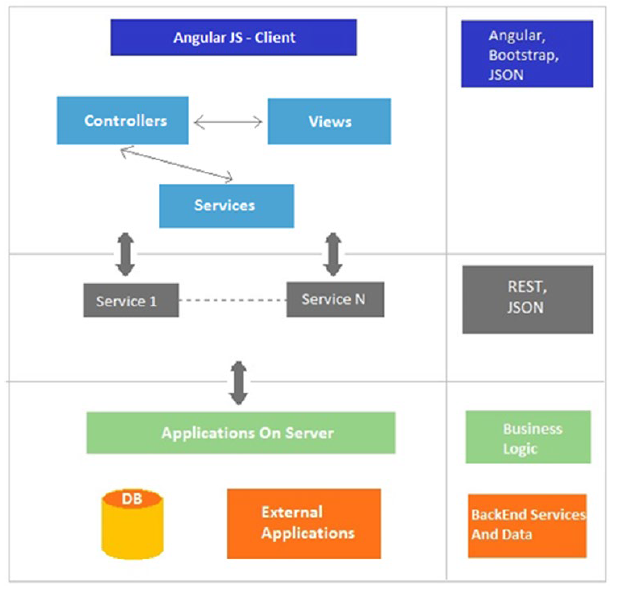
\includegraphics[width=16cm]{../imgs/ejemplos/webapp-arq.png}
			\caption{Arquitectura de aplicaciones web modernas}
			\label{figure:webapp-arq}
		\end{figure}
		
		 
	
	\subsection{Bootstrap}
		Bootstrap es un framework CSS que, facilita la creación se sitios web
		Responsive Web Design. Bootstrap viene con un conjunto de componentes de
		interfaz web listos para usar y una guía de estilos bastante completa,
		también provee grillas para el correcto maquetado de una web profesional.
		
		\begin{figure}[H]
		    \centering
			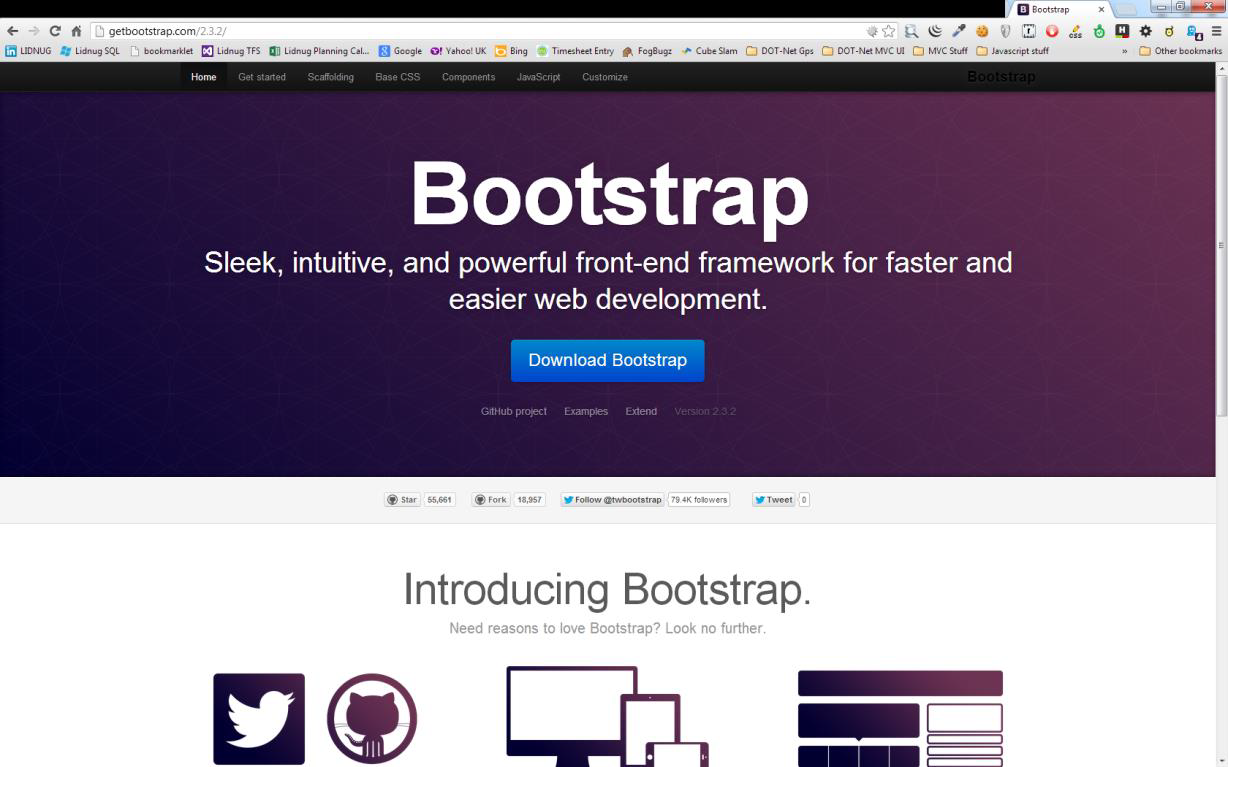
\includegraphics[width=17cm]{../imgs/ejemplos/bootstrap.png}
			\caption{Sitio Web de Bootstrap}
		\end{figure}
		
	
	\subsection{AngularJS}
		AngularJS es un framework de código abierto, soportado por Google. AngularJS
		permite a los desarrolladores crear aplicaciones web SPA (Single Page Applications), lo
		que facilita la experiencia de usuario, al no tener que cargar la
		aplicación web completa dos ó más veces.\\\
		
		A diferencia del las aplicaciones web SPA, en las aplicaciones
		web tradicionales (como se ilustra en la figura
		\ref{figure:carga-tradicional}), un cliente web hace una petición al servidor
		y éste responde con toda la página web completa; luego, el usuario hace click
		en un enlace interno, el servidor vuelve a cargar la página web completa
		y se produce un retraso en la carga de la página, lo que produce una mala
		experiencia de usuario.\footnote{Fuente de la imagen:
		\href{https://www.codeschool.com/course/shaping-up-with-angularjs}
		{https://www.codeschool.com/course/shaping-up-with-angularjs}} \\\
		
		\begin{figure}[H]
		    \centering
			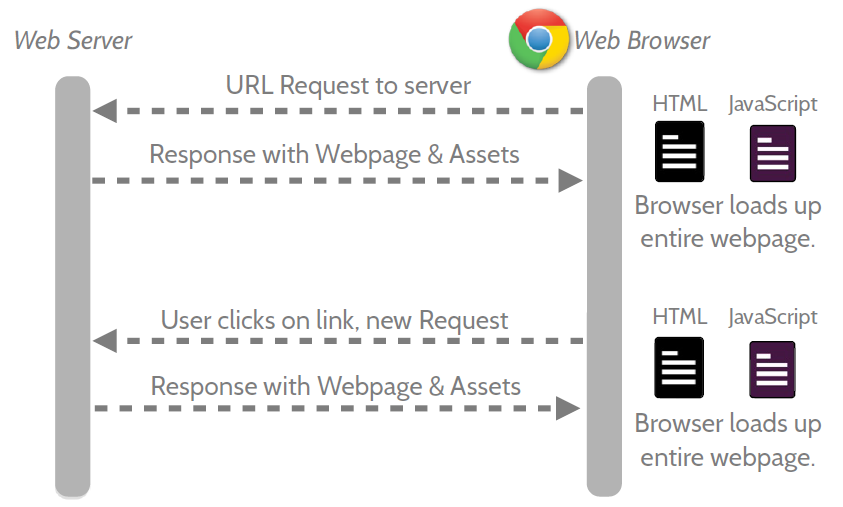
\includegraphics[width=18cm]{../imgs/ejemplos/1.png}
			\caption{Carga de página tradicional}
			\label{figure:carga-tradicional}
		\end{figure}
		
		
		En las aplicaciones SPA, el cliente solicita una web y el servidor
		inicialmente sirve la aplicación web completa (una sola vez); luego, el
		usuario hace click en un enlace interno, el servidor solo responde con el recurso
		solicitado, más no con la página web completa. En la figura
		\ref{figure:carga-spa} se muestra esta interacción.\footnote{Fuente de la imagen: 
		\href{https://www.codeschool.com/course/shaping-up-with-angularjs}
		{https://www.codeschool.com/course/shaping-up-with-angularjs}}
		
		\newpage
		\begin{figure}[H]
		    \centering
			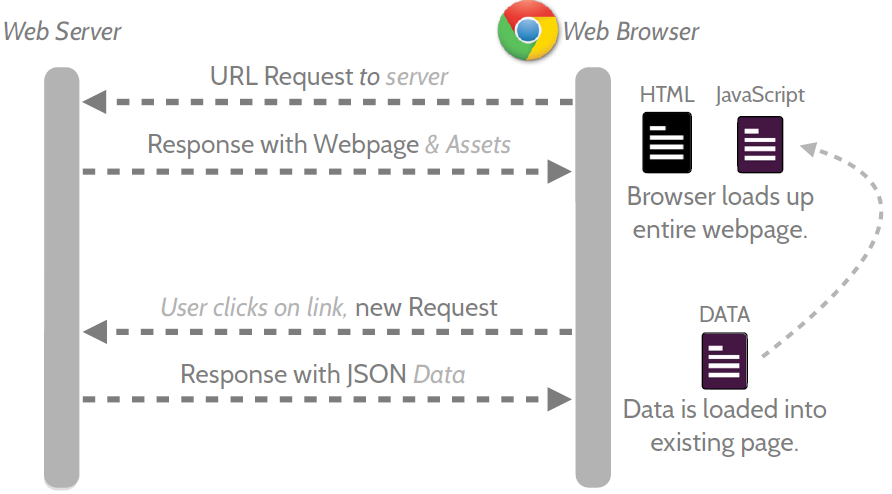
\includegraphics[width=18cm]{../imgs/ejemplos/2.png}
			\caption{Carga de página SPA}
			\label{figure:carga-spa}
		\end{figure}
		
		\newpage
		\subsubsection{Componentes}
			AngularJS ofrece una estructura modular y escalable para
			construir aplicaciones web, figura \ref{figure:angularjs-comp}.
			
			\begin{figure}[H]
			    \centering
				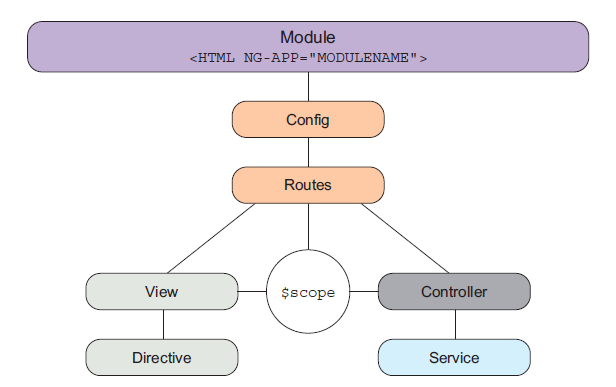
\includegraphics[width=18cm]{../imgs/ejemplos/angularjs-comp.png}
				\caption{Componentes de AngularJS}
				\label{figure:angularjs-comp}
			\end{figure}
			
			\begin{table}[H]
				\begin{tabular}{|p{2.75cm}|p{14cm}|} \hline
					 & \\
					\textit{\bfseries Componente} & \textit{\bfseries Propósito} \\
					 & \\ \hline
					 
					 & \\
					Module & Sirve como un contenedor que ayuda a organizar el
					código. Los Módulos pueden contener submódulos, haciendo fácil la
					composición de funcionalidades dentro de una aplicación web.\\
					 & \\
					 
					Config & El bloque de configuración permite ejecutar código javascript
					antes de que le aplicación se ejecute.\\
					Routes & Permite definir rutas para navegar a estados específicos de la
					aplicación.\\
					& \\
					
					View & La vista es la plantilla HTML que mostrará la aplicación.\\
					& \\
					
					\$scope & El \$scope es básicamente el pegamento entre la vista y el
					contralador\\
					& \\
					
					Controller & El controlador es responsable de la definición de métodos y
					propiedades. La vista es quien interactúa con el controlador.\\
					& \\
					
					Directive & Es una extensión de una vista, permite crear
					elementos HTML personalizados que encapsulan comportamientos.\\
					& \\
					Service & Proporcionan funcionalidades comunes a una aplicación.\\
					& \\ \hline
				\end{tabular}
				\caption{Resumen de componentes AngularJS}
			\end{table}
			
		\subsubsection{Arquitectura}
			AngularJS sigue una arquitectura MVC (Modelo-Vista-Controlador) para crear
			aplicaciones web. MVC es un patrón de
			arquitectura que separa los datos, lógica y
			presentación (figura \ref{figure:mvc}). Propuesto por
			\textit{Trygve Reenskaug} y después fue implementaado en el lenguaje de
			programación Smalltalk en los sententa \cite{scott1spa}.
			
			\begin{figure}[H]
			    \centering
				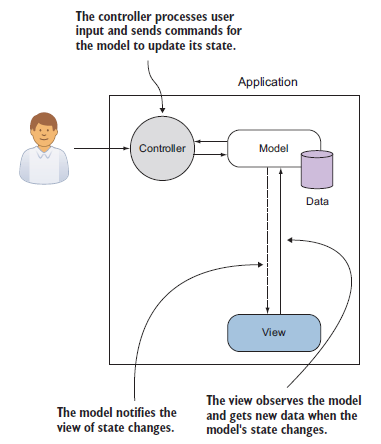
\includegraphics[width=16cm]{../imgs/ejemplos/mvc.png}
				\caption{Arquitectura Modelo-Vista-Controlador}
				\label{figure:mvc}
			\end{figure}
			
		
	\subsection{NodeJS y ExpressJS}
		NodeJS no es un lenguaje de programación, es una plataforma capaz de ejecutar
		aplicaciones complejas escritas en Javascript; se ejecuta en el lado del
		servidor como cualquier otro lenguaje (Java, Python, Ruby, etc).
		Para el sistema fue usado como un proxy, y a la vez como un servidor estático.\\\
		
		NodeJS está construido sobre el motor de javascript V8 creado por Google.
		NodeJS posee varias librerías escritas en C, junto con módulos para la
		manipulación de datos binarios, puede acceder a funciones del sistema
		operativo, etc. Éstas librerías permiten a NodeJS acceder a archivos, ejecutar
		comandos del sistema, escuchar/responder a peticiones de red.\\\
		
		La figura \ref{figure:nodejs-comp} muestra los componentes principales de
		NodeJS:
		
		\begin{figure}[H]
		    \centering
			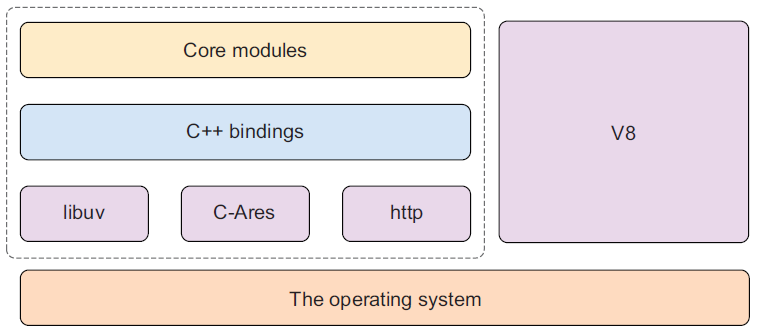
\includegraphics[width=16cm]{../imgs/ejemplos/nodejs-comp.png}
			\caption{Componentes de NodeJS}
			\label{figure:nodejs-comp}
		\end{figure}
		
		
		
		ExpressJS es un framework web para NodeJS. Proporciona una API sencilla de
		utilizar, y agiliza el desarrollo de proyectos backend.
	\newpage
	
	\subsection{Spring y Spring Boot}
		Spring es un framework java para el desarrollo de aplicaciones a nivel
		empresarial, inició como una alternativa liviana al estándar {\bf Java
		Enterprise Edition (JEE)}. Spring ofrece características como inyección de
		dependencias y un modelo de programación orientada a aspectos.\\\
		
		\subsubsection{Arquitectura}
			Como se muestra en la figura \ref{figure:spring-comp}, la arquitectura de
			Spring es modular, lo que permite elegir únicamente los módulos que
			necesitemos, sin necesidad de traer el framework completo.
		
			\begin{figure}[H]
			    \centering
				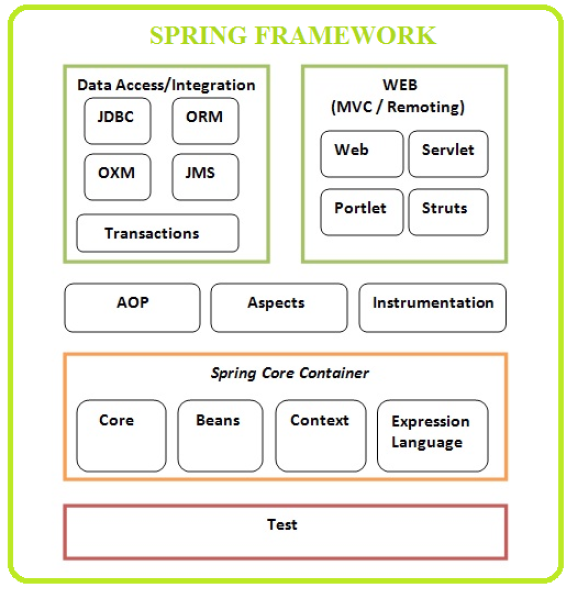
\includegraphics[width=14cm]{../imgs/ejemplos/spring-comp.png}
				\caption{Arquitectura de Spring Framework}
				\label{figure:spring-comp}
			\end{figure}
			
			
			
			\begin{table}[H]
				\begin{tabular}{|p{4.75cm}|p{12cm}|} \hline
					 & \\
					\textit{\bfseries Módulo} & \textit{\bfseries Propósito} \\
					 & \\ \hline
					 
					 & \\
					Core Container & Proporciona características de IoC (Inverción de Control)
					e Inyección de dependencias.\\
					 & \\
					 
					AOP \& Instrumentation & Proporciona un mecanimso para introducir nuevas
					funcionalidades a un código existente sin modificar su diseño.\\
					& \\
					
					Data Access/Integration & Se encarga de gestionar el acceso a bases de
					datos en una aplicación.\\
					& \\
					
					Web & Prorporciona un buen soporte para la creación de aplicaciones web
					robustas.\\
					& \\
					
					Test & Ayuda a realizar pruebas unitarias y de integración usando JUnit y
					TestNG.\\
					& \\
					
					& \\ \hline
				\end{tabular}
				\caption{Módulos de Spring}
			\end{table}
			
			
			
		
		Spring brinda muchas facilidades a la hora de programar, pero la
		configuración es un tanto compleja. Spring Boot simplifica toda las
		configuraciones iniciales para comenzar un proyecto web de manera rápida.
		Cabe mencionar que Spring Boot no es una herramienta ni una alternativa a Spring,
		es un proyecto que necesita de Spring para facilitarnos la vida.\\\
		
		Spring Boot trae algo de magia al desarrollo de aplicaciones con Spring.
		Existen cuatro características fundamentales:
		
		\begin{itemize}
		  \item {\bf Configuración Automática:} {Spring Boot proporciona de manera
		  automática funcionalidades a nuestro proyecto.}
		  
		  \item {\bf Dependencias Iniciales:} {De acuerdo al tipo de proyecto, Spring
		  Boot facilita las librerias necesarias para iniciar un proyecto.}
		  
		  \item {\bf Interfaz de Línea de Comandos:} {Esta característica opcional
		  permite escribir trozos de código directamente en la terminal e ir
		  probando funcionalidades.}
		  
		  \item {\bf Actuador (\textit{The Actuator}):} {Muestra características de
		  una aplicación en tiempo de ejecución.}
		\end{itemize}
		
		La página oficial (http://start.spring.io) del proyecto Spring Boot ofrece un
		asistente para la creación de proyectos utilizando maven o gradle:
		
		\begin{figure}[H]
		    \centering
			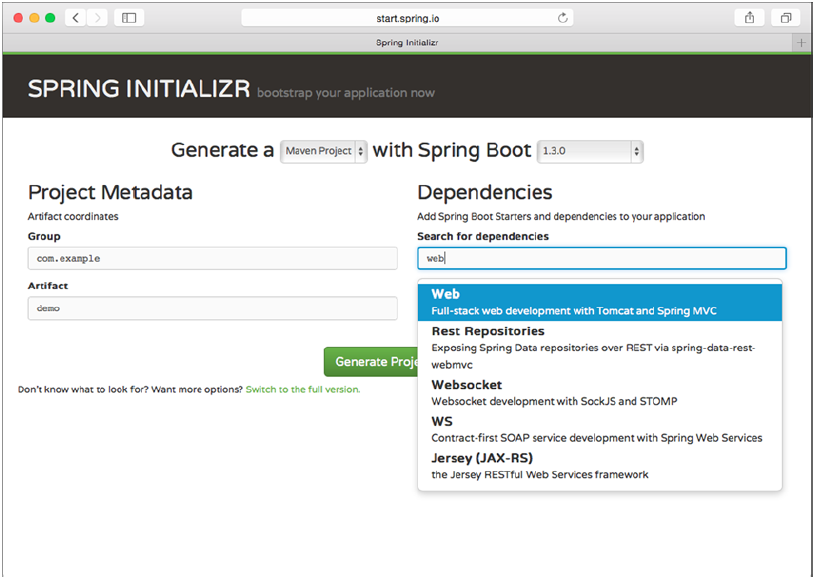
\includegraphics[width=14cm]{../imgs/ejemplos/spring-boot.png}
			\caption{Asistente de Spring Initializr}
			\label{figure:spring-boot}
		\end{figure}
		
		Después de generar el proyecto, obtenemos un archivo .zip el cual podemos
		importar a IDEs como Eclipse o NetBeans. La estructura de un proyecto Spring
		Boot es muy sencilla como se muestra en la figura
		\ref{figure:spring-boot-est}.

		\begin{figure}[H]
		    \centering
			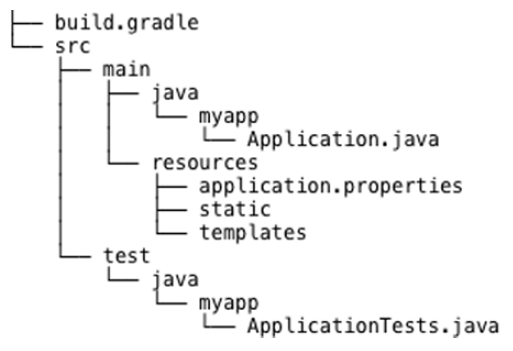
\includegraphics[width=10cm]{../imgs/ejemplos/spring-boot-est.png}
			\caption{Estructura de un proyecto Spring Boot}
			\label{figure:spring-boot-est}
		\end{figure}
		
		El ecosistema Spring cuenta con otros proyectos que vale la pena conocer, a
		continuación se listan algunos de ellos:
		
		\begin{table}[H]
			\begin{tabular}{|p{4.75cm}|p{12cm}|} \hline
				 & \\
				\textit{\bfseries Proyecto} & \textit{\bfseries Descripción} \\
				 & \\ \hline
				 
				 & \\
				Spring Cloud & Proporciona un conjunto de herramientas para sistemas
				distribuidos. Útil para la construcción y despliegue de microservicios.\\
				 & \\
				 
				Spring Data & Proporciona una aproximación consistente para el acceso a
				bases de datos: Relacionales, no-relacionales, map-reduce, etc.\\
				& \\
				
				Spring Batch & Simplifica y optimiza el procesamiento de altos volúmenes
				de operaciones en bloque.\\
				& \\
				
				Spring Security & Proteje nuestras aplicaciones de una forma simple.
				Soporte para autenticación y autorización.\\
				& \\
				
				Spring Hateoas & Simplifica la creación de servicios RESTful y sigue el
				pricipio HATEOAS.\\
				& \\
				
				Spring Rest Docs & Documenta automáticamente nuestros servicios RESTful.\\
				& \\
				
				Spring Social & Conecta fácilmente nuestras aplicaciones con APIs de
				terceros: Facebook, Twitter, Linkedin y más.\\
				& \\
				
				& \\ \hline
			\end{tabular}
			\caption{Proyectos del ecosistema Spring}
		\end{table}
		